% Snapshot of the instructor's course seed. One third-party reading reference was omitted.
\documentclass{article}
\usepackage{graphicx}
\usepackage{amsmath}
\usepackage{amssymb}
\usepackage{listings}
\usepackage[margin=1in]{geometry}
\usepackage{xcolor}
\usepackage{tikz}
\usetikzlibrary{shapes, arrows, positioning, calc, shadows}
\usepackage{tcolorbox}
\usepackage{cite}

% Define colors for syntax highlighting
\definecolor{codegreen}{rgb}{0,0.6,0}
\definecolor{codegray}{rgb}{0.5,0.5,0.5}
\definecolor{codepurple}{rgb}{0.58,0,0.82}
\definecolor{backcolour}{rgb}{0.95,0.95,0.92}

% Python style for highlighting
\lstdefinestyle{pythonstyle}{
    backgroundcolor=\color{backcolour},
    commentstyle=\color{codegreen},
    keywordstyle=\color{magenta},
    numberstyle=\tiny\color{codegray},
    stringstyle=\color{codepurple},
    basicstyle=\ttfamily\footnotesize,
    breakatwhitespace=false,
    breaklines=true,
    captionpos=b,
    keepspaces=true,
    numbers=left,
    numbersep=5pt,
    showspaces=false,
    showstringspaces=false,
    showtabs=false,
    tabsize=2
}
\lstset{style=pythonstyle}

\title{Lecture 7-?: RNN bridghe to Attention\\From Memory Overload to Dynamic Focus}
\author{Deep Learning Class}
\date{\today}

\begin{document}
\maketitle

\section{Introduction: A Story of Forgetting}

\begin{tcolorbox}[colback=blue!5!white, colframe=blue!50!black, title=Today's Journey]
We'll discover how a simple insight---``what if the model could look back at the input while writing?''---revolutionized deep learning and led to ChatGPT, BERT, and modern AI.
\end{tcolorbox}



















\section{Part 4: Building Attention---From Intuition to Code}

\subsection{The Teaching Version (Simple Loops)}

Let's implement exactly what we just described, step by step:

\begin{lstlisting}[language=Python, caption=Attention: The Intuitive Version]
def attention_simple(decoder_state, encoder_states):
    """
    The simplest possible attention - exactly matching our 3 steps
    This is teaching code - we'll optimize it later!
    """

    # Step 1: "Where should I look?" - Calculate alignment scores
    scores = []
    for encoder_state in encoder_states:
        # How similar is what I need (decoder_state)
        # to what's available (encoder_state)?
        score = torch.dot(decoder_state, encoder_state)
        scores.append(score)

    print(f"Raw scores (interest levels): {scores}")
    # Example: [0.8, 2.1, 0.5] - high interest in position 2

    # Step 2: "How much should I focus?" - Convert to percentages
    # Softmax makes them sum to 1.0 (100%)
    # Stack preserves dtype, device, and autograd history.
    attention_weights = torch.softmax(torch.stack(scores), dim=0)

    print(f"Attention weights (focus %): {attention_weights}")
    # Example: [0.20, 0.70, 0.10] - 70% focus on position 2

    # Step 3: "What do I take away?" - Weighted combination
    context = torch.zeros_like(decoder_state)
    for i, weight in enumerate(attention_weights):
        context += weight * encoder_states[i]

    # context is now a focused blend of the input information!
    return context, attention_weights

# Let's see it in action!
decoder_state = torch.randn(512)  # What I'm looking for
encoder_states = [torch.randn(512) for _ in range(5)]  # Available info

context, weights = attention_simple(decoder_state, encoder_states)
\end{lstlisting}

\subsection{Visualizing Attention Live}

Here's what makes attention truly magical---we can watch it work:

\begin{lstlisting}[language=Python, caption=Live Attention Visualization]
def show_attention_live(source_words, target_words, all_attention_weights):
    """
    ASCII visualization showing the 'flashlight' moving during translation
    """

    for step, target_word in enumerate(target_words):
        print(f"\n=== Step {step+1}: Generating '{target_word}' ===")
        print("Where is the model looking?\n")

        weights = all_attention_weights[step]

        for src_word, weight in zip(source_words, weights):
            # Create a visual bar (like a flashlight intensity)
            bar_length = int(weight * 30)
            bar = "=" * bar_length
            intensity = "DIM " if weight < 0.2 else "BRIGHT!" if weight > 0.5 else "medium"

            print(f"  {src_word:10s} [{weight:.2f}] {bar} {intensity}")

        time.sleep(1)  # Pause to see the movement

# Example output when translating "Le chat mange":
"""
=== Step 1: Generating 'The' ===
Where is the model looking?

  Le         [0.75] ====================== BRIGHT!
  chat       [0.20] ======                 medium
  mange      [0.05] =                      DIM

=== Step 2: Generating 'cat' ===
Where is the model looking?

  Le         [0.10] ===                    DIM
  chat       [0.85] ========================= BRIGHT!
  mange      [0.05] =                      DIM
"""
\end{lstlisting}

\subsection{The Efficient Version (Matrix Operations)}

Now that we understand the concept, let's see why real implementations use matrix operations:

\begin{lstlisting}[language=Python, caption=Attention: The PyTorch Way]
def attention_efficient(decoder_state, encoder_states):
    """
    Same 3 steps, but using matrix ops for GPU efficiency
    This processes all comparisons in parallel!
    """

    # encoder_states: [seq_length, hidden_size]
    # decoder_state: [hidden_size]

    # Step 1: All dot products at once using matrix multiplication
    # Instead of a loop, we do ALL comparisons simultaneously
    scores = torch.matmul(encoder_states, decoder_state)

    # Step 2: Softmax (same as before)
    attention_weights = torch.softmax(scores, dim=0)

    # Step 3: Weighted sum using matrix multiplication
    # Instead of a loop, blend everything at once
    context = torch.matmul(attention_weights, encoder_states)

    return context, attention_weights

# Why is this better?
# - Loop version: 100 sequential operations for 100 words
# - Matrix version: 1 parallel operation for 100 words
# On a GPU, this is 10-100x faster!
\end{lstlisting}

\section{Part 5: Seeing is Believing---Attention Patterns}

\subsection{The Alignment Matrix}

When we collect all attention weights across all decoding steps, we get a beautiful visualization:

\begin{center}
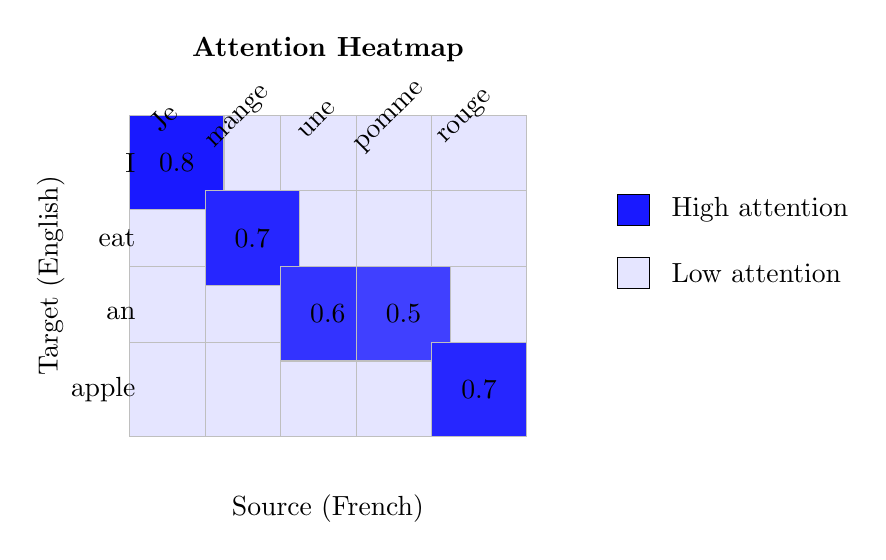
\begin{tikzpicture}[scale=0.8]
    % Create heatmap grid
    \foreach \i in {0,...,3} {
        \foreach \j in {0,...,4} {
            \pgfmathsetmacro{\opacity}{10}
            \node[draw=gray!50, minimum width=1.2cm, minimum height=1.2cm,
                  fill=blue!\opacity] (cell\i\j) at (\j*1.2, -\i*1.2) {};
        }
    }

    % Highlight diagonal pattern (word alignment)
    \node[draw=gray!50, minimum width=1.2cm, minimum height=1.2cm,
          fill=blue!90] at (0, 0) {0.8};
    \node[draw=gray!50, minimum width=1.2cm, minimum height=1.2cm,
          fill=blue!85] at (1.2, -1.2) {0.7};
    \node[draw=gray!50, minimum width=1.2cm, minimum height=1.2cm,
          fill=blue!80] at (2.4, -2.4) {0.6};
    \node[draw=gray!50, minimum width=1.2cm, minimum height=1.2cm,
          fill=blue!75] at (3.6, -2.4) {0.5};
    \node[draw=gray!50, minimum width=1.2cm, minimum height=1.2cm,
          fill=blue!85] at (4.8, -3.6) {0.7};

    % Labels
    \foreach \word [count=\i from 0] in {Je, mange, une, pomme, rouge} {
        \node[rotate=45, anchor=south] at (\i*1.2, 0.5) {\word};
    }

    \foreach \word [count=\i from 0] in {I, eat, an, apple} {
        \node[anchor=east] at (-0.5, -\i*1.2) {\word};
    }

    % Title and axes
    \node[font=\bfseries] at (2.4, 1.8) {Attention Heatmap};
    \node at (2.4, -5.5) {Source (French)};
    \node[rotate=90] at (-2, -1.8) {Target (English)};

    % Legend
    \draw[fill=blue!90] (7, -1) rectangle (7.5, -0.5);
    \node[anchor=west] at (7.7, -0.75) {High attention};
    \draw[fill=blue!10] (7, -2) rectangle (7.5, -1.5);
    \node[anchor=west] at (7.7, -1.75) {Low attention};
\end{tikzpicture}
\end{center}

Notice the diagonal pattern! The model learned the word alignments without any explicit supervision.

\subsection{Different Attention Patterns}

Attention can learn various patterns depending on the task:

\begin{lstlisting}[language=Python, caption=Analyzing Attention Patterns]
def classify_attention_pattern(attention_matrix):
    """
    Identify what kind of attention pattern the model learned
    """

    # Calculate metrics
    diagonal_strength = measure_diagonal(attention_matrix)
    entropy = calculate_entropy(attention_matrix)
    max_peak = attention_matrix.max()

    if diagonal_strength > 0.7:
        return "MONOTONIC: Direct word-to-word translation"
    elif entropy > 2.0:
        return "DISTRIBUTED: Combining information from many sources"
    elif max_peak > 0.8:
        return "FOCUSED: Strong attention to specific keywords"
    else:
        return "MIXED: Complex attention pattern"

# Examples of what we might see:
# - "The red car" -> "La voiture rouge": Non-monotonic (word reordering)
# - "It's raining" -> "Il pleut": Focused (phrasal translation)
# - Technical text: Often monotonic (preserves order)
\end{lstlisting}

\section{Part 6: Common Misconceptions}

\begin{tcolorbox}[colback=yellow!5!white, colframe=yellow!50!black, title=Is Attention Actually Memory?]
\textbf{No!} This is a common confusion. Let's clarify:
\begin{itemize}
\item \textbf{Memory:} Storage of information (like encoder hidden states)
\item \textbf{Attention:} The mechanism to ACCESS that memory selectively
\end{itemize}
Think of it this way: A library (memory) contains all the books. A librarian (attention) helps you find the right book when you need it.
\end{tcolorbox}

\begin{tcolorbox}[colback=yellow!5!white, colframe=yellow!50!black, title=What Makes Attention ``Soft''?]
\textbf{Soft = Weighted Average} instead of hard selection:
\begin{itemize}
\item \textbf{Hard Attention:} Pick ONLY position 3 (not differentiable!)
\item \textbf{Soft Attention:} 70\% position 3, 20\% position 2, 10\% position 4
\end{itemize}
Soft attention is differentiable, so we can train it with backpropagation!
\end{tcolorbox}


\subsection{The Revolution It Started}

\begin{center}
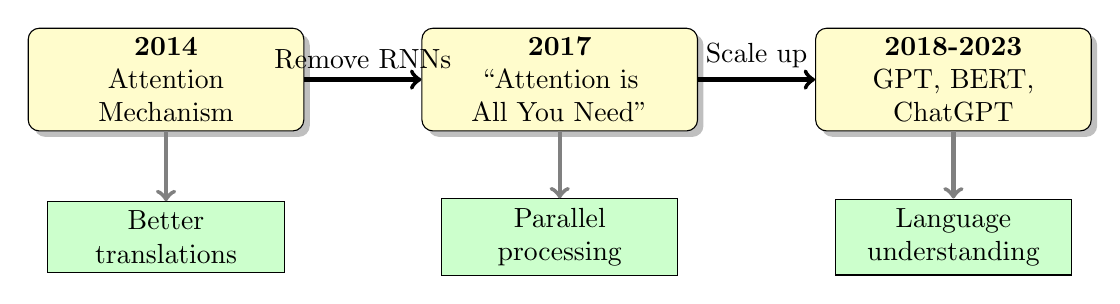
\begin{tikzpicture}[
    node distance=2cm,
    innovation/.style={rectangle, rounded corners, draw, fill=yellow!20,
                      minimum width=3.5cm, minimum height=1.2cm, align=center,
                      drop shadow},
    impact/.style={rectangle, draw, fill=green!20, minimum width=3cm,
                   minimum height=0.8cm, align=center},
    arrow/.style={->, ultra thick}
]
    % Timeline
    \node[innovation] (attention) at (0, 0) {\textbf{2014}\\Attention\\Mechanism};
    \node[innovation] (transformer) at (5, 0) {\textbf{2017}\\``Attention is\\All You Need''};
    \node[innovation] (gpt) at (10, 0) {\textbf{2018-2023}\\GPT, BERT,\\ChatGPT};

    \draw[arrow] (attention) -- (transformer) node[midway, above] {Remove RNNs};
    \draw[arrow] (transformer) -- (gpt) node[midway, above] {Scale up};

    % Impacts
    \node[impact] (impact1) at (0, -2) {Better\\translations};
    \node[impact] (impact2) at (5, -2) {Parallel\\processing};
    \node[impact] (impact3) at (10, -2) {Language\\understanding};

    \draw[arrow, gray] (attention) -- (impact1);
    \draw[arrow, gray] (transformer) -- (impact2);
    \draw[arrow, gray] (gpt) -- (impact3);
\end{tikzpicture}
\end{center}

\section{Hands-On Exercise: Build Your Own Attention}

\subsection{Exercise 1: Implement Temperature Control}

\begin{lstlisting}[language=Python, caption=Exercise: Attention Temperature]
def attention_with_temperature(decoder_state, encoder_states, temperature=1.0):
    """
    TODO: Implement attention with temperature control

    Temperature controls how "focused" the attention is:
    - High temp (>1): More distributed attention (explore more)
    - Low temp (<1): More focused attention (exploit the best)
    - Temp = 0: Hard attention (pick only the maximum)

    Hint: Divide scores by temperature before softmax
    """
    # Your code here:
    scores = torch.matmul(encoder_states, decoder_state)

    # TODO: Apply temperature scaling here
    # scores = scores / temperature

    attention_weights = torch.softmax(scores, dim=0)
    context = torch.matmul(attention_weights, encoder_states)
    return context, attention_weights

# Test with different temperatures and visualize the difference!
\end{lstlisting}

\subsection{Exercise 2: Attention Visualization Game}

\begin{lstlisting}[language=Python, caption=Interactive Attention Game]
def attention_guessing_game(model, sentence_pairs):
    """
    Game: Predict where the model will attend!
    """
    for source, target in sentence_pairs:
        print(f"\nTranslating: '{source}' -> '{target}'")
        print("Where will the model look when generating each word?")

        # Get user predictions
        user_predictions = []
        for i, target_word in enumerate(target.split()):
            guess = input(f"  Generating '{target_word}' - which source word? ")
            user_predictions.append(guess)

        # Get actual attention
        _, attention_weights = model.translate(source)

        # Compare and score
        print("\nResults:")
        visualize_attention_comparison(user_predictions, attention_weights)

# Try it with:
# - "The red car" -> "La voiture rouge"  (reordering!)
# - "Thank you" -> "Merci"  (many-to-one!)
\end{lstlisting}

\section{Summary: The Power of Looking Back}

\begin{tcolorbox}[colback=green!5!white, colframe=green!50!black, title=What We Learned Today]
\begin{enumerate}
\item \textbf{The Problem:} Seq2seq models forget early information (the bottleneck)
\item \textbf{The Insight:} Let the decoder look back at all encoder states (like keeping a book open)
\item \textbf{The Mechanism:} Three simple steps---Compare, Focus, Combine
\item \textbf{The Impact:} Attention revolutionized NLP and led to modern AI
\end{enumerate}

\textbf{Remember:} Attention is just a learnable way to say ``what should I look at right now?''
\end{tcolorbox}

\subsection{Preview: Next Week's Mind-Blowing Question}

We've seen that attention is incredibly powerful. It lets our model dynamically access information. But we still have RNNs doing the encoding and decoding sequentially.

\begin{center}
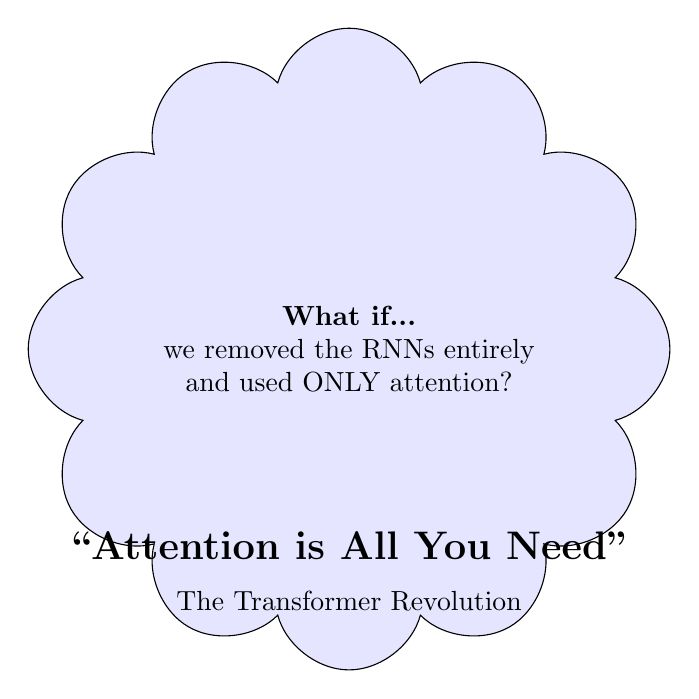
\begin{tikzpicture}[
    thought/.style={cloud, draw, fill=blue!10, minimum width=4cm,
                   minimum height=2cm, align=center, cloud puffs=12}
]
    \node[thought] at (0, 0) {\textbf{What if...}\\we removed the RNNs entirely\\and used ONLY attention?};

    \node[font=\Large\bfseries] at (0, -2.5) {``Attention is All You Need''};
    \node at (0, -3.2) {The Transformer Revolution};
\end{tikzpicture}
\end{center}

Next week: We'll see how this radical idea gave us ChatGPT, and why ``self-attention'' might be the key to artificial intelligence.

\section{Practice Problems}

\begin{enumerate}
\item \textbf{Conceptual:} Why does attention help more with long sentences than short ones?

\item \textbf{Implementation:} Modify the simple attention to use cosine similarity instead of dot product. How does this change the behavior?

\item \textbf{Analysis:} Given attention weights [0.1, 0.7, 0.2], and encoder states representing [``cat'', ``eats'', ``fish''], what information would the context vector primarily contain?

\item \textbf{Debugging:} Your attention weights are all nearly equal (uniform). What might be wrong? (Hint: think about the magnitude of your dot products)

\item \textbf{Extension:} Implement ``coverage penalty''---penalize the model for attending to the same positions repeatedly. Why might this help?
\end{enumerate}

\section*{References}

\begin{thebibliography}{9}
\bibitem{bahdanau2014neural}
Bahdanau, D., Cho, K., \& Bengio, Y. (2014).
Neural machine translation by jointly learning to align and translate.
\textit{arXiv preprint arXiv:1409.0473}.

\bibitem{luong2015effective}
Luong, M. T., Pham, H., \& Manning, C. D. (2015).
Effective approaches to attention-based neural machine translation.
\textit{EMNLP 2015}.

\bibitem{vaswani2017attention}
Vaswani, A., et al. (2017).
Attention is all you need.
\textit{NeurIPS 2017}.
\end{thebibliography}

\section*{Appendix A: Mathematical Details}

For those interested in the formal mathematics, here are the attention equations:

\textbf{Bahdanau (Additive) Attention:}
\begin{align}
e_{ti} &= v^T \tanh(W_s s_{t-1} + W_h h_i) \\
\alpha_{ti} &= \frac{\exp(e_{ti})}{\sum_{j=1}^T \exp(e_{tj})} \\
c_t &= \sum_{i=1}^T \alpha_{ti} h_i
\end{align}

\textbf{Luong (Multiplicative) Attention:}
\begin{align}
\text{score}(s_t, h_i) &= \begin{cases}
s_t^T h_i & \text{(dot)} \\
s_t^T W h_i & \text{(general)} \\
v^T \tanh(W[s_t; h_i]) & \text{(concat)}
\end{cases}
\end{align}

But remember: the intuition is more important than the equations!

\section*{Appendix B: Resources}

\begin{itemize}
\item \textbf{Interactive Demo:} \texttt{https://jalammar.github.io/visualizing-attention/}
% Third-party reading reference omitted from the public source snapshot.
\item \textbf{Original Papers:} Start with Bahdanau et al. (2014)---it's surprisingly readable!
\item \textbf{Video:} ``Attention in Neural Networks'' by Yannic Kilcher
\end{itemize}




\section{The Memory Bottleneck Problem}

When we built our first seq2seq models, we made a bold assumption: we could compress an entire source sequence into a single fixed-dimensional vector. This is the \textbf{bottleneck} that eventually led us to discover attention.

% \begin{figure}[h]
% \centering
% \begin{tikzpicture}[scale=0.8]
%     % Encoder
%     \foreach \i in {1,...,5} {
%         \node[draw, circle, minimum size=0.8cm, fill=blue!20] (enc\i) at (\i*1.5, 0) {$h_\i$};
%         \node[above] at (enc\i.north) {$x_\i$};
%     }

%     % Connections in encoder
%     \foreach \i in {1,...,4} {
%         \pgfmathtruncatemacro{\j}{\i+1}
%         \draw[->, thick] (enc\i) -- (enc\j);
%     }

%     % The bottleneck
%     \node[draw, rectangle, minimum width=1.5cm, minimum height=1cm, fill=red!30] (bottleneck) at (10, 0) {$c$};
%     \draw[->, thick, red, rotat] (enc5) -- (bottleneck) node[midway, above, rotate = 0] {compress};

%     % Decoder
%     \foreach \i in {1,...,4} {
%         \node[draw, circle, minimum size=0.8cm, fill=green!20] (dec\i) at (10.5+\i*1.5, 0) {$s_\i$};
%         \node[above] at (dec\i.north) {$y_\i$};
%     }

%     % Connections in decoder
%     \draw[->, thick, red] (bottleneck) -- (dec1);
%     \foreach \i in {1,...,3} {
%         \pgfmathtruncatemacro{\j}{\i+1}
%         \draw[->, thick] (dec\i) -- (dec\j);
%     }

%     \node[below=0.5cm] at (3.5, -1) {Encoder};
%     \node[below=0.5cm] at (bottleneck.south) {Fixed Memory};
%     \node[below=0.5cm] at (13, -1) {Decoder};
% \end{tikzpicture}
% \caption{The vanilla seq2seq architecture: Everything flows through a single bottleneck vector $c$}
% \end{figure}

\begin{tcolorbox}[colback=yellow!5!white, colframe=orange!50!black, title=The Compression Problem]
Think of this like trying to describe an entire movie in a single tweet. For a short clip, maybe that works. But for a three-hour epic? You're going to lose crucial details. This is exactly what happens when sequences get long—BLEU scores drop dramatically after 30-40 tokens.
\end{tcolorbox}

\section{From One Vector to a Bank of Vectors: The Key Insight}

The breakthrough came when we realized: why throw away all those intermediate encoder states? Let's keep them all! This transforms our latent space from a single vector into a \textbf{sequence of memory slots}.

\begin{figure}[h]
\centering
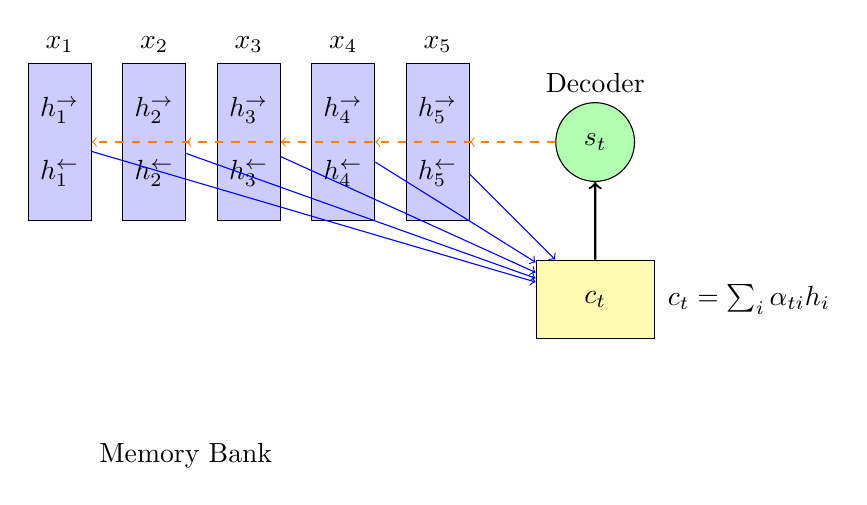
\begin{tikzpicture}[scale=0.8]
    % Encoder states (memory bank)
    \foreach \i in {1,...,5} {
        \node[draw, rectangle, minimum width=0.8cm, minimum height=2cm, fill=blue!20] (mem\i) at (\i*1.5, 0) {};
        \node at (\i*1.5, 0.5) {$h_\i^{\rightarrow}$};
        \node at (\i*1.5, -0.5) {$h_\i^{\leftarrow}$};
        \node[above] at (mem\i.north) {$x_\i$};
    }

    % Current decoder state
    \node[draw, circle, minimum size=1cm, fill=green!30] (decoder) at (10, 0) {$s_t$};
    \node[above] at (decoder.north) {Decoder};

    % Attention connections
    \foreach \i in {1,...,5} {
        \draw[->, dashed, orange] (decoder) -- (mem\i);
    }

    % Context vector
    \node[draw, rectangle, minimum width=1.5cm, minimum height=1cm, fill=yellow!30] (context) at (10, -2.5) {$c_t$};

    % Weighted sum
    \foreach \i in {1,...,5} {
        \draw[->, blue] (mem\i) -- (context);
    }

    \draw[->, thick] (context) -- (decoder);

    \node[below=0.5cm] at (3.5, -4) {Memory Bank};
    \node[right] at (11, -2.5) {$c_t = \sum_{i} \alpha_{ti} h_i$};
\end{tikzpicture}
\caption{The attention mechanism: The decoder can access all encoder states, not just the last one}
\end{figure}

Andrew Ng motivates the same idea with a human translator: a translator works through
a sentence in aligned pieces instead of compressing the entire source into memory and
then producing the target from that single recollection.

\section{Naming the Components: Query, Keys, and Values}

Now let's give proper names to what we've been doing. When the decoder needs to generate the next word, it asks a question (query) to the memory bank:

\begin{itemize}
    \item \textbf{Query} ($q_t$): ``What am I looking for?'' — The decoder's current hidden state $s_{t-1}$
    \item \textbf{Keys} ($K$): ``What's available to match against?'' — All encoder hidden states $\{h_1, ..., h_T\}$
    \item \textbf{Values} ($V$): ``What information to retrieve?'' — Also the encoder states (or transformations of them)
\end{itemize}

\begin{tcolorbox}[colback=blue!5!white, colframe=blue!50!black, title=The Attention Computation]
\begin{align}
\text{score}(q_t, k_i) &= \frac{q_t^T W k_i}{\sqrt{d_k}} \quad \text{(scaled dot-product)} \\
\alpha_{ti} &= \frac{\exp(\text{score}(q_t, k_i))}{\sum_j \exp(\text{score}(q_t, k_j))} \\
c_t &= \sum_i \alpha_{ti} v_i
\end{align}
Note: The $\sqrt{d_k}$ scaling keeps gradients stable (temperature control).
\end{tcolorbox}

\subsection{Shape Cheat Sheet}

\begin{tcolorbox}[colback=gray!5!white, colframe=gray!50!black, title=Tensor Shapes Quick Reference]
For batch size $B$, sequence length $T$, model dimension $d$, heads $h$, per-head dimension $d_k = d/h$:
\begin{itemize}
    \item $Q, K, V: [B, T, d] \rightarrow [B, h, T, d_k]$ (after projection and reshape)
    \item Attention scores: $[B, h, T, T]$ (every position attends to every position)
    \item Attention weights: $[B, h, T, T]$ (after softmax)
    \item Output per head: $[B, h, T, d_k]$
    \item Final output: $[B, T, d]$ (after concatenation and projection)
\end{itemize}
\end{tcolorbox}

\subsection{Attention Masking: Handling Padding and Causality}

\begin{tcolorbox}[colback=red!5!white, colframe=red!50!black, title=Critical: Masking in Attention]
Two types of masks are essential for correct attention:
\begin{enumerate}
    \item \textbf{Padding Mask}: Ignore padded tokens in variable-length sequences
    \item \textbf{Causal Mask}: Prevent positions from attending to future positions (decoder)
\end{enumerate}
\end{tcolorbox}

\begin{figure}[h]
\centering
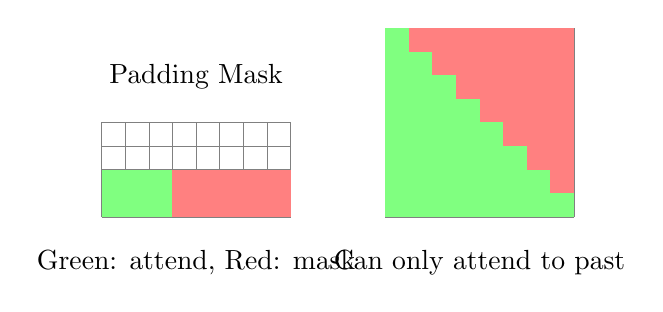
\begin{tikzpicture}[scale=0.6]
    % Padding mask
    \node[above] at (2, 2.5) {Padding Mask};
    \draw[step=0.5cm,gray,very thin] (0,0) grid (4,2);
    % Valid positions
    \foreach \x in {0,1,2} {
        \foreach \y in {0,1} {
            \fill[green!50] (\x*0.5,\y*0.5) rectangle (\x*0.5+0.5,\y*0.5+0.5);
        }
    }
    % Padded positions
    \foreach \x in {3,4,5,6,7} {
        \foreach \y in {0,1} {
            \fill[red!50] (\x*0.5,\y*0.5) rectangle (\x*0.5+0.5,\y*0.5+0.5);
        }
    }

    % Causal mask
    \begin{scope}[xshift=6cm]
        \node[above] at (2, 2.5) {Causal Mask};
        \draw[step=0.5cm,gray,very thin] (0,0) grid (4,4);
        % Lower triangular
        \foreach \i in {0,...,7} {
            \foreach \j in {0,...,\i} {
                \fill[green!50] (\j*0.5,3.5-\i*0.5) rectangle (\j*0.5+0.5,4-\i*0.5);
            }
        }
        % Upper triangular (masked)
        \foreach \i in {0,...,7} {
            \foreach \j in {\i,...,7} {
                \pgfmathtruncatemacro{\jplus}{\j+1}
                \ifnum\jplus>8\else
                    \ifnum\j>\i
                        \fill[red!50] (\j*0.5,3.5-\i*0.5) rectangle (\j*0.5+0.5,4-\i*0.5);
                    \fi
                \fi
            }
        }
    \end{scope}

    \node[below] at (2, -0.5) {Green: attend, Red: mask};
    \node[below] at (8, -0.5) {Can only attend to past};
\end{tikzpicture}
\caption{Padding mask for variable-length sequences and causal mask for autoregressive generation}
\end{figure}

\begin{lstlisting}[language=Python]
def masked_softmax(scores, valid_lens=None, causal=False):
    """Apply padding and/or causal masking before softmax"""
    if valid_lens is not None:
        # Create padding mask
        positions = torch.arange(scores.shape[-1], device=scores.device)
        mask = positions.unsqueeze(0) < valid_lens.to(scores.device).unsqueeze(-1)
        # [B, 1, 1, T_k] broadcasts over heads and query positions.
        scores = scores.masked_fill(~mask[:, None, None, :], -1e6)

    if causal:
        # Create causal mask (lower triangular)
        seq_len = scores.shape[-1]
        causal_mask = torch.tril(
            torch.ones(seq_len, seq_len, dtype=torch.bool, device=scores.device)
        )
        scores = scores.masked_fill(causal_mask == 0, -1e6)

    return torch.softmax(scores, dim=-1)
\end{lstlisting}

\section{Attention as Linear Transformation in Latent Space}

One useful geometric picture is a learned linear transformation in latent space that
aligns queries with keys. A general learned matrix may rotate, scale, shear, or project;
it need not be a pure rotation. When we compute $q^T W k$, we are effectively:

\begin{figure}[h]
\centering
\begin{tikzpicture}[scale=1.2]
    % Original space
    \draw[->] (-2,0) -- (2,0) node[right] {dim 1};
    \draw[->] (0,-2) -- (0,2) node[above] {dim 2};

    % Query vector
    \draw[->, thick, blue] (0,0) -- (1.5,1) node[right] {$q$};

    % Key vector
    \draw[->, thick, red] (0,0) -- (0.5,1.5) node[above] {$k$};

    % Transformed space
    \begin{scope}[xshift=6cm]
        \draw[->] (-2,0) -- (2,0) node[right] {dim 1'};
        \draw[->] (0,-2) -- (0,2) node[above] {dim 2'};

        % After transformation
        \draw[->, thick, blue] (0,0) -- (1.5,1) node[right] {$Wq$};
        \draw[->, thick, red] (0,0) -- (1.5,1.2) node[above] {$k$};

        % Show alignment
        \draw[<->, green, thick] (0.2,0.13) arc (35:40:2);
        \node[green] at (2,-1) {aligned!};
    \end{scope}

    \draw[->, thick, purple] (2.5,0) -- (3.5,0) node[midway, above] {$W$};

    \node at (0,-3) {Original Space};
    \node at (6,-3) {Transformed Space};
\end{tikzpicture}
\caption{Attention scoring as a learned linear transformation that aligns query and key vectors}
\end{figure}

The matrix $W$ learns a linear transformation of the query space so that pairs useful
to the task receive high dot products. Calling the transformation a rotation is only
a picture; an unconstrained $W$ may also scale, shear, or project.




\section{Key Takeaways}

\begin{tcolorbox}[colback=blue!5!white, colframe=blue!75!black, title=The Big Picture]
\begin{enumerate}
    \item \textbf{Attention is content-based memory access}: Instead of forcing everything through a fixed-size pipe, we maintain a memory bank and learn to retrieve what's relevant.

    \item \textbf{Q, K, V are natural concepts}: They emerge naturally when we formalize ``looking up relevant information'' — query what you want, match against keys, retrieve values.

    \item \textbf{Linear transformations create semantic spaces}: The weight matrices in attention learn to project queries and keys into spaces where similarity means semantic relevance.

    \item \textbf{Multi-head = multiple perspectives}: Different projections capture different types of relationships in parallel.

    \item \textbf{Self-attention removes the sequential bottleneck}: By letting every position attend to every other position directly, we enable massive parallelization.
\end{enumerate}
\end{tcolorbox}



\section{GoodRead: Essential Papers}

\begin{tcolorbox}[colback=gray!5!white, colframe=gray!75!black, title=Recommended Reading List]
\textbf{Foundational Papers:}
\begin{enumerate}
    \item \textbf{Bahdanau et al. (2014)} — ``Neural Machine Translation by Jointly Learning to Align and Translate''
    \begin{itemize}
        \item The paper that introduced attention to NMT
        \item Start here — it's surprisingly readable!
    \end{itemize}

    \item \textbf{Luong et al. (2015)} — ``Effective Approaches to Attention-based Neural Machine Translation''
    \begin{itemize}
        \item Introduces ``dot-product attention'' (simpler than Bahdanau's additive attention)
        \item Compares different attention variants systematically
    \end{itemize}

    \item \textbf{Vaswani et al. (2017)} — ``Attention Is All You Need''
    \begin{itemize}
        \item The Transformer paper — read it after understanding basic attention
        \item Focus on Sections 3.1-3.3 for the core ideas
    \end{itemize}
\end{enumerate}

\textbf{Understanding and Visualization:}
\begin{enumerate}
    \setcounter{enumi}{3}
    \item \textbf{Olah \& Carter (2016)} — ``Attention and Augmented Recurrent Neural Networks'' (Distill)
    \begin{itemize}
        \item Beautiful interactive visualizations
        \item Great for building intuition
    \end{itemize}

    \item \textbf{Weng (2018)} — ``Attention? Attention!'' (Blog post)
    \begin{itemize}
        \item Comprehensive tutorial covering all attention variants
        \item Excellent mathematical notation and clarity
    \end{itemize}
\end{enumerate}

\textbf{Extensions and Applications:}
\begin{enumerate}
    \setcounter{enumi}{5}
    \item \textbf{Shaw et al. (2018)} — ``Self-Attention with Relative Position Representations''
    \begin{itemize}
        \item How to incorporate position information beyond simple embeddings
    \end{itemize}

    \item \textbf{Devlin et al. (2018)} — ``BERT: Pre-training of Deep Bidirectional Transformers''
    \begin{itemize}
        \item See how self-attention enables bidirectional context
        \item The beginning of the pre-training era
    \end{itemize}

    \item \textbf{Dosovitskiy et al. (2020)} — ``An Image is Worth 16x16 Words''
    \begin{itemize}
        \item Vision Transformers — attention beyond sequences!
        \item Shows the generality of the attention mechanism
    \end{itemize}
\end{enumerate}

\textbf{For the Mathematically Inclined:}
\begin{enumerate}
    \setcounter{enumi}{8}
    \item \textbf{Chorowski et al. (2015)} — ``Attention-Based Models for Speech Recognition''
    \begin{itemize}
        \item More complex attention mechanisms (location-aware, hybrid)
        \item Good for understanding attention variants
    \end{itemize}

    \item \textbf{Lin et al. (2017)} — ``A Structured Self-attentive Sentence Embedding''
    \begin{itemize}
        \item Multi-hop attention and attention regularization
        \item Interesting theoretical insights
    \end{itemize}
\end{enumerate}
\end{tcolorbox}



\end{document}
